%This is a LaTeX template for homework assignments
\documentclass{article}
\usepackage[utf8]{inputenc}
\usepackage{amsmath}
\usepackage{graphicx}
\usepackage{enumitem}


\begin{document}

\title{EMET1001: ASSIGNMENT WEEK 1}
\author{ZEMING WANG\\U6114134}
\date{\today}
\maketitle

%---------------------%
\subsection*{PROBLEM 2}
\vspace{1em}
\begin{equation*}
    F(x) = 1 + \frac{4x}{x^2+4}
\end{equation*}
\vspace{1em}

\begin{enumerate}[label=(\alph*)]
\item Compute F(0), F(-2), F(2), and F(3). 
\begin{equation*}
\begin{aligned}
    F(0) &= 1 + \frac{4 \cdot 0}{0^2 + 4} = 1 \\
    F(-2) &= 1 + \frac{4 \cdot (-2)}{(-2)^2 + 4} = 0 \\
    F(2) &= 1 + \frac{4 \cdot 2}{2^2 + 4} = 2 \\
    F(3) &= 1 + \frac{4 \cdot 3}{3^2 + 4} = \frac{25}{13} \\
\end{aligned}
\end{equation*}

\item What happens to $F(x)$ when $x$ becomes large positive or negative? 
\begin{equation*}
    F(x) = 1 + \frac{4x}{x^2+4} = 1 + \frac{4}{x + \frac{4}{x}}
\end{equation*}
When $x$ becomes very large, no matter positive or negative, 
it drives $\dfrac{4}{x}$ to $0$, and $\dfrac{4}{x + \frac{4}{x}}$ also becomes $0$.
Therefore, $F(x)$ will end up with the value $1$.

\item Give a rough sketch of the graph of F. \\\\
The graph roughly looks like this:\\\\
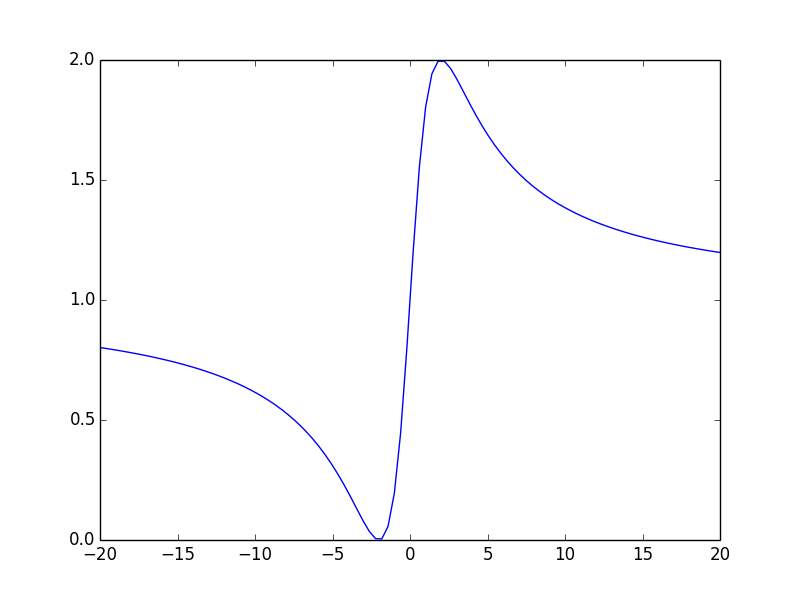
\includegraphics[scale=0.6]{figure_1}
\end{enumerate}

%---------------------%
\subsection*{PROBLEM 4}
\vspace{1em}
Find the domains of the following functions:
\vspace{1em}
\begin{enumerate}[label=(\alph*),itemsep=4ex,partopsep=1ex]
\item $f(x)=\sqrt{x^2 - 1}$ \\\\
\begin{equation*}
    x^2 - 1 \geq 0\ \textrm{(it is under square root and cannot be negative)} \implies x^2 \geq 1 \implies x \geq 1, \textrm{or}\ x \leq -1
\end{equation*}
\\Therefore, the domain is $(-\infty, -1]\cup[1, +\infty)$.

\item $g(x)=\dfrac{1}{\sqrt{x - 4}}$ \\\\
\begin{equation*}
    x - 4 > 0\ \textrm{(it is the denominator and thus cannot be zero)} \implies x > 4
\end{equation*}
\\Therefore, the domain is $(4, +\infty)$.

\item $h(x)=\sqrt{(x-3)(5-x)}$ \\\\
\begin{equation*}
    (x-3)(5-x) \geq 0 \implies
        \begin{cases} x-3 \geq 0\\5-x \geq 0 \end{cases},\ 
        \textrm{or} \
        \begin{cases} x-3 \leq 0\\5-x \leq 0 \end{cases}
        \implies 3 \leq x \leq 5
\end{equation*}
\\Therefore, the domain is $[3, 5]$.
\end{enumerate}


%---------------------%
\subsection*{PROBLEM 7}
\vspace{1em}
Find the equations for the following straight lines:
\vspace{1em}

\begin{enumerate}[label=(\alph*),itemsep=4ex,partopsep=1ex]
\item $L1$ passes throught $(-2,3)$ and has a slope of $-3$. \\\\
\textbf{SOLUTION:}\\\\
Applying the foluma: $$y - y_1 = a(x - x_1)$$
the line equation is: $$y - 3 = -3(x-(-2))$$
which is:$$3x+y+3=0$$

\item $L2$ passes through $(-3, 5)$ and $(2,7)$. \\\\
\textbf{SOLUTION:}\\\\
The slope of the line is: $$a = \frac{7-5}{2-(-3)} = \frac{2}{5}$$
so the line is: $$y - 5 = \frac{2}{5}(x - (-3)) $$
which is: $$2x - 5y + 31 = 0$$

\item $L3$ passes through $(a,b)$ and $(2a,3b)$ (suppose $a \neq 0$). \\\\
\textbf{SOLUTION:}\\\\
The slope is: $$a=\frac{3b-b}{2a-a}=\frac{2b}{a}$$
so the line is: $$y - b=\frac{2b}{a}(x - a)$$
which is: $$2bx - ay -ab = 0$$

\end{enumerate}


%---------------------%
\subsection*{PROBLEM 10}
\vspace{1em}
Find the equation for the parabola $y=ax^2 + bx + c$ that passes through the 
three points $(1,-3)$, $(0,-6)$, and $(3,15)$.
\vspace{1em}
\\\\\textbf{SOLUTION:}\\\\
Assign the three points to $(x,y)$ in the equation:
\begin{equation*}
\begin{aligned}
-3 &= a + b + c \\
-6 &= c \\
15 &= 9a + 3b + c
\end{aligned}
\end{equation*}
solve the equations, we get:
\begin{equation*}
\begin{aligned}
a &= 2\\
b &= 1\\
c &= -6
\end{aligned}
\end{equation*}
So the parabola equation is: $$y = 2x^2 + x - 6$$

%---------------------%
\subsection*{PROBLEM 21}

\vspace{1em}
Solve for $t$.
\vspace{1em}

\begin{enumerate}[label=(\alph*),itemsep=4ex,partopsep=1ex]

\item $x = e^{at+b}$ \\\\
\textbf{SOLUTION:}\\\\
Take natural logarithm on both side of the equation:
$$\ln{x} = at + b, x > 0 $$
sove for $t$:
$$t = \frac{\ln{x} - b}{a}, x > 0$$

\item $e^{-at} = \dfrac{1}{2}$ \\\\
\textbf{SOLUTION:}\\\\
Take logarithm on both side of the equation:
$$-at = \ln{\frac{1}{2}} \implies at = \ln{2} $$
which gives:
$$t = \frac{\ln{2}}{a}$$

\item $\dfrac{1}{\sqrt{2\pi}}e^{-\dfrac{t^2}{2}} = \dfrac{1}{8}$ \\\\\\
\textbf{SOLUTION:}\\\\
The original equation is equivalent to:
$$ e^{-\frac{t^2}{2}} = \frac{\sqrt{2\pi}}{8} $$
taking logrithm on both side gives:
$$-\frac{t^2}{2} = \ln{\frac{\sqrt{2\pi}}{8}} \implies t = \sqrt{-2\ln{\frac{\sqrt{2\pi}}{8}}}$$
which is essentially:
$$ t = \sqrt{\ln{\frac{32}{\pi}}}$$

\end{enumerate}

\end{document}